%-----------------------------------------------------------------------------%
\chapter{\babDua}
%-----------------------------------------------------------------------------%
Pada bab ini akan dijelaskan teori - teori yang akan digunakan dalam penelitian ini. Penjelasan teori yang terdapat dibab ini merupakan hasil dari pembelajaran literatur.
%-----------------------------------------------------------------------------%
\section{Teori Perancangan Game}
	\subsection{Definisi Game}
	\textit{Game} merupakan media interaksi yang memadukan beberapa elemen. Elemen yang dimaksud berupa gambar, tulisan, suara dan lain - lain. Menurut Rogers (2010) dalam bukunya yang berjudul "\textit{Level Up:The Guide To Great Video Game Design}", \textit{game} adalah aktivitas yang memiliki peraturan, tujuan, dan minimal satu pemain. Menurut Schell (2015) dalam buku "\textit{The Art of Game Design}", \textit{game} adalah "\textit{an exercise of voluntary control systems, in which there is a contest between powers, confined by rules in order to produce a disequilibrial outcome}".
	\linebreak\linebreak
	Menurut buku "\textit{Rules of Play}", Salen dan Zimmerman (2004), beberapa peneliti telah mengutarakan definisi dari \textit{game}. Salen dan Zimmerman mengatakan \textit{game} adalah sebuah konflik yang dibuat sedemikian rupa, terdapat peraturan didalamnya dan sebuah hasil. David Parlett mengatakan ada dua elemen penting yaitu \textit{Ends} (akhir dari  \textit{game} yang telah didefinisikan) dan \textit{Means} (cara seorang pemain untuk mencapai tujuan game tersebut).
	\subsection{Kategori Game}
	Jumlah game saat ini sudah meningkat setiap tahunnya. Setiap game memiliki ciri khas yang berbeda - beda. Untuk memudahkan dalam mengenali jenis \textit{game}, jurnalis, pemain, dan developer sepakat untuk mengklasifikasi \textit{game} sesuai dengan katagorinya. Herz (1997) mengelompokkan \textit{game} menjadi :
	\begin{itemize}
		\item \textit{Action Game}
			\subitem Genre ini mengutamakan kemampuan fisik dari pemainnya. Kemampuan yang dituntut dalam memainkan genre ini berupa koordinasi mata dengan reflek dari pemainnya. Pemain akan menjadi pemeran utama yang akan melakukan begitu banyak aksi didalamnya.
		\item \textit{Role-Playing Game}
			\subitem Sebuah genre dimana pemain akan memeran seorang karakter dalam \textit{game} yang memiliki sebuah cerita yang harus diselesaikan.
		\item \textit{Simulation Game}
			\subitem Genre yang mengambil sebuah kejadian dari kehidupan nyata dan diubah menjadi bentuk \textit{game}. Sebagai contoh permainan mesimulasi sebagai batu, dalam \textit{game} tersebut pemain akan memerankan sebagai batu yang hanya bisa diam dan terombang - ambing.
		\item \textit{Strategy Game}
			\subitem Sebuah Genre dimana pemain mengendalikan sebuah atau beberapa unit dan mengatur cara agar dapat memenangkan permainan tersebut.
		\item \textit{Sports Game}
			\subitem Genre ini sejenis dengan simulasi, genre ini lebih memfokuskan tentang kejadian pada dunia olahraga.
		\item \textit{Idle Game}
			\subitem Genre ini meminimkan aksi yang dilakukan oleh pemain. Contoh \textit{game} dari genre ini adalah "Cookie Clicker" yang hanya mengharuskan pemain untuk menekan layar pada perangkat kerasnya.
	\end{itemize}
	
	\subsection{Elemen Game}
	Terdapat beberapa elemen dalam \textit{game} yang sangat penting dan menjadi rujukan untuk meningkatkan performa dari permainan yang dibuat oleh \textit{developer}. Schell (2015) menuliskan elemen yang ada dalam sebuah permainan dalam buku "\textit{The Art of Game Design} sebagai berikut :
	\begin{itemize}
		\item Estetika
			\subitem Elemen untuk menampilkan gambar, suara dan suasana dalam permainan tersebut. Dengan menampilkan hal - hal tersebut maka pengalaman user dalam memainkan permainan tersebut akan meningkat.
		\item Teknologi
			\subitem Elemen ini merupakan struktur bagaimana permainan ini dibuat dalam pengembangan \textit{game}.
		\item Mekanik
			\subitem Mekanik adalah sebuah elemen dari game yang berperan sebagai prosedur dan peraturan dari permainan tersebut. Mekanik mendeskripsikan tujuan dari game tersebut, bagaimana pemain bisa mencapai tujuan tersebut, konsekuensi apa yang diterima.
		\item Naratif
			\subitem Naratif adalah sebuah elemen dari game yang berperan sebagai cerita dari game tersebut. Naratif ini bisa dibagi menjadi Linear \& Prescripted, dan Branching \& Emergent. Linear \& Prescripted dimaksudkan sebagai naratif yang hanya memiliki satu cerita atau makna yang sudah dipersiapkan sebelumnya, sedangkan Branching \& Emergent dimaksudkan sebagai naratif yang memiliki lebih dari satu cabang cerita sehingga setiap pemain dapat memiliki cerita dan makna yang berbeda, tidak dipersiapkan mungkin bisa diatasi dengan Artificial Intelligence yang memperhatikan input dari pemain.
	\end{itemize}
	
\section{Teori Pembelajaran}
	\subsection{Definisi Pembelajaran}
		Untuk mengetahui bagaimana cara korelasi antara pembelajaran dan \textit{game}, maka kita harus mengetahui terlebih dahulu bagaimana definisi dari pembelajaran secara umum. terdapat 4 aspek dalam teori pembelajaran yaitu Behaviourist,Cognitivist, Humanist, dan Social \& Situational (Kirriemuir \& Mcfarlane 2008).
		%\tablename{Definisi Pembelajaran}
		\begin{table}
			\centering
			\caption{Perbandingan setiap aspek dari beberapa teori pembelajaran}
			\label{tab:tab1}
			\begin{tabular}{| c | c | c | c | c |}
				\hline
				Aspek & \textit{Behaviourist} & \textit{Cognitivistt} & \textit{Humanist} & \multicolumn{1}{p{2cm}|}{\textit{Social and Situational}} \\
				\hline
				\multicolumn{1}{|p{2cm}|}{\raggedright Proses Pembelajaran} & \multicolumn{1}{p{2.5cm}|}{\raggedright Penggantian perilaku} & \multicolumn{1}{p{2.5cm}|}{\raggedright Semua proses terjadi di dalam kepala pelajar seperti (insight, information processing, memory, perception)} & \multicolumn{1}{p{2.5cm}|}{\raggedright Perkembangan terhadap potensial pribadi} & \multicolumn{1}{p{2.5cm}|}{\raggedright Interaksi dan observasi di dalam grup} \\
				\hline
				\multicolumn{1}{|p{2cm}|}{Tujuan edukasi} & \multicolumn{1}{p{2.5cm}|}{\raggedright Mencari perubahan perilaku kepada arah yang ditentukan} & \multicolumn{1}{p{2.5cm}|}{\raggedright Melakukan pengembangan kemampuan untuk belajar yang lebih baik} & \multicolumn{1}{p{2.5cm}|}{Mandiri} & \multicolumn{1}{p{2.5cm}|}{\raggedright Partisipasi yang penuh terhadap komunitas} \\
				\hline
				\multicolumn{1}{|p{2cm}|}{Sumber Pembelajaran} & \multicolumn{1}{p{2.5cm}|}{\raggedright Sumber eksternal dan tugas} & \multicolumn{1}{p{2.5cm}|}{\raggedright Membuat koneksi terhadap pengetahuan yang sudah diketahui} & \multicolumn{1}{p{2.5cm}|}{\raggedright Emosi, perilaku, dan pemikiran} & \multicolumn{1}{p{2.5cm}|}{\raggedright Hubungan antara orang dan lingkungan} \\
				\hline
			\end{tabular}
		\end{table}
	
	\subsection{Bloom's Taxonomy with revision (Anderson \& Krathwohl, 2001)}
	Bloom's taxonomy merupakan suatu taksonomi yang diciptakan pertama kali oleh beberapa peneliti yang diketuai oleh Bloom ( Bloom et all 1956) yang dikenal dalam artikelnya yang berjudul \textit{"Bloom Taxonomy of the Cognitive Domain"}. Pada awalnya terdapat enam tingkat yang dikenal dengan Bloom's Taxonomy yaitu Knowledge, Comprehension, Application, Analysis, Synthesis, dan Evaluation. 
	\linebreak \linebreak
	Terdapat revisi dari Bloom's taxonomy yang dikerjakan oleh Anderson \& Krathwohl (2001) , dengan perubahan menjadi :
	\begin{itemize}
		\item \textit{Remember}
			\subitem Tingkatan terbawah dari Bloom's taxonomy ini merupakan mengingat, yang memiliki penjelasan tentang bagaimana setelah pengertian maka langkah selanjutnya adalah untuk mengingat beberapa pengertian yang telah dihasilkan pada tahap sebelumnya. Melakukan mapping terhadap pengetahuan yang sudah diketahui dengan satu dan lainnya.
		\item \textit{Understand}
			\subitem Tingkatan kelima merupakan \textit{understand} atau pengertian, yang memiliki penjelasan tentang bagaimana setelah menerapkan maka langkah selanjutkan untuk pengertian konsep, meringkas materi tersebut, melakukan klasifikasi terhadap materi tersebut, mendalami prinsip, dan membandingkan beberapa materi dengan materi lainnya untuk sebagai pengertian.
		\item \textit{Apply}
			\subitem Tingkatan keempat merupakan menerapkan, yang memiliki penjelasan tentang bagaimana penerapan prosedur yang sesuai dari tugas yang memiiki kemiripan satu dan lainnya. Misalkan kita sudah mengetahui prosedur yang harus dilakukan dalam suatu masalah, maka kita bisa mencoba menerapkan prosedur yang sama kepada tugas yang mirip dengan yang kita telah selesaikan.
		\item \textit{Analyze}
			\subitem Tingkatan ketiga merupakan analisis, yang memiliki penjelasan tentang bagaimana membedakan materi yang relevan maupun tidak relevan dan menentukan porsi kepentingan dari suatu materi yang diberikan ataupun ditemukan.
		\item \textit{Evaluate}
			\subitem Tingkatan kedua merupakan \textit{evaluate} atau evaluasi, yang memiliki penjelasan tentang bagaimana uji coba terhadap konsistensi, kelayakan, maupun efektifitas dalam prinsip maupun prosedur. Selanjutnya melakukan kritik terhadap konsistensi, kelayakan, dan efektifitas dari prinsip maupun posedur. Kritik terebut berdasar kepada uji coba yang layak.
		\item \textit{Create}
			\subitem Tingkat paling atas dari Bloom's taxonomy ini merupakan \textit{create} atau membuat, yang memiliki penjelasan tentang bagaimana menentukan beberapa hipotesis terhadap beberapa kriteria, melakukan desain prosedur untuk menyelesaikan tugas tertentu. Lalu membuat innovasi untuk menyelesaikan tugas tertentu.
		
	\end{itemize}
	Terdapat penjelasan lebih lanjut yang dikerjakan oleh Anderson dan Karthwohl (2001) mengenai Knowledge Dimension atau Dimensi Pengetahuan yang berbasis pada Bloom's Taxonomy seperti:
	\begin{table}
		\centering
		\huge
		\caption{Dimensi Pengetahuan}
		\label{tab:tab1}
		\begin{tabular}{| p{1.2cm} | p{1.2cm} | p{1.2cm} | p{1.2cm} | p{1.2cm} | p{1.2cm} | p{1.2cm} | p{1.2cm} |}
			\hline
			\multicolumn{2}{| p{3cm} |}{\multirow{2}{*}{\scriptsize Knowledge Dimension}} & \multicolumn{6}{| c |}{\small Dimensi Proses Kognitif} \\
			\multicolumn{2}{|c|}{}  & \scriptsize Remember & \scriptsize Understand & \scriptsize Apply & \scriptsize Analyze & \scriptsize Evaluate & \scriptsize Create \\
			\hline
			\scriptsize Factual Knowledge & \scriptsize Terminologi, Komponen \& Element & \raggedright \scriptsize List nama Label map &\raggedright \scriptsize  Intepretasi suatu materi di buku & \raggedright \scriptsize Memakai Algoritma & \raggedright \scriptsize Kategori kata & \raggedright \scriptsize Kritik Artikel & \scriptsize Membuat cerita pendek \\
			\hline
			\scriptsize Conceptual Knowledge & \scriptsize Kategori, Prinsip, Teori & \raggedright \scriptsize Definisi tingkatan konsep &\raggedright \scriptsize  Deskripsi sesuai pemahaman & \raggedright \scriptsize Tuliskan objektif konsep & \raggedright \scriptsize Perbedaan setiap konsep & \raggedright \scriptsize Kritik dari objektif konsep & \scriptsize Membuat suatu klasifikasi baru \\
			\hline
			\scriptsize Procedural Knowledge & \scriptsize Kemampuan Spesifik, Teknik  \& kriteria penggunaan & \raggedright \scriptsize List langkah yang digunakan &\raggedright \scriptsize  Memahami proses problem solving dengan kata kata sendiri & \raggedright \scriptsize Menggunakan proses problem solving untuk menyelesaikan permasalahan & \raggedright \scriptsize Melakukan komparasi beberapa teknik & \raggedright \scriptsize Kritik terhadap kelayakan dalam teknik yang digunakan & \scriptsize Membuat suatu pendekatan baru dalam penyelesaian masalah \\
			\hline
			\scriptsize Meta-Cognitive Knowledge & \scriptsize Pengetahuan terhadap diri sendiri & \raggedright \scriptsize List elementt dari cara pembelajaran mandiri &\raggedright \scriptsize  Melakukan deksripsi terhadap implikasi dari cara pembelajaran tersebut & \raggedright \scriptsize Mengembangkan suatu kemampuan pembelajaran dari cara pembelajaran tersebut & \raggedright \scriptsize Melakukan komparasi terhadap dimensi cara pembelajaran & \raggedright \scriptsize Kritik terhadap kelayakan dalam beberapa cara pembelajaran dengan cara pembelajaran yang digunakan & \scriptsize Membuat suatu cara baru dalam pembelajaran \\
			\hline
		\end{tabular}
	\end{table}
	
	
	\subsection{\textit{Expectation Effect}}
	Terdapat suatu teori dalam pembelajaran yaitu \textit{Pygmalion Effect} atau disebut juga \textit{Expectation Effect}. \textit{Expectation Effect} tersebut menjelaskan tentang bagaimana suatu ekspektasi dari seorang guru terhadap siswa, dapat mempengaruhi prestasi siswa tersebut. Teori tersebut pertama kali dipelopori oleh seorang psikolog dari Harvard bernama Robert Rosenthal yang bekerja sama dengan beberapa kepala sekolah untuk menjalankan suatu eksperimen di beberapa sekolah dasar pada tahun  1964 - 1965. Dalam penelitiannya tersebut Robert melakukan klasifikasi terhadap siswa yang memiliki potensi akademis yang tinggi, tetapi tidak terlihat berprestasi pada nilai akademisnya atau disebut juga dengan "late bloomer". Robert Rosenthal ingin meneliti efek apakah yang terjadi ketika seseorang diberikan ekspektasi yang positif kepada dirinya, yang merupakan berkebalikan dengan apa yang dilakukan oleh Jane Elliot, dimana melaksanakan hal yang mirip dengan yang dilakukan Robert Rosenthal tetapi perbedaannya adalah seseorang diberikan suatu ekspektasi yang negatif kepada dirinya.
	\linebreak \linebreak
	Terdapat beberapa teori penting dalam \textit{Expectation Effect} yang bisa menjadi basis pendukung dari \textit{Game Based Learning}, yaitu:
	\begin{enumerate}
		\item \textit{Halo Effect}
			\subitem Teori ini dipelopori oleh Edward Thorndike pada tahun 1920, merupakan studi yang beliau lanjutkan dari studi yang dia buat pada tahun 1915. Edward Thorndike melakukan wawancara pada saat perang dunia, dimana dia menanyakan kepada atasan militer bagaimana atasan tersebut melakukan evaluasi setiap anggota tentara yang mereka pimpin. Aspek yang Thorndike tanyakan adalah kualitas fisik, intelektual, kepemimpinan, maupun secara pribadi. Maksud dari penelitian ini adalah bagaimana penilaian dari satu karakteristik mempengaruhi karakteristik yang lain. Teori dari halo effect ini menjelaskan tentang bagaimana kesan dari satu aspek dalam teknologi memberikan suatu makna terhadap bagaimana teknologi tersebut digunakan.
		\item \textit{Hawthorne Effect}
			\subitem Teori ini dipelopori oleh Henry A. Landsberger pada tahun 1958, ketika sedang melakukan analisa terhadap eksperimen pada perusahaan Hawtrhone Works yang pada saat itu adalah sebuah perusahaan listrik di daerah Chicago, Amerika Serikat. Pada saat itu, perusahaan tersebut ingin mempelajari apakah pekerja mereka akan lebih produktif bekerja di tempat gelap atau terang. Studi tersebut membuktikan bahwa ketika periode perubahan dari gelap ke terang dilakukan terjadi peningkatan kerja, tetapi ketika eksperimen berakhir maka tidak terjadi peningkatan sama sekali. Teori ini menemukan bahwa peningkatan kerja tersebut adalah sebuah hasil efek motivasi dari pekerja karena tertarik dengan teori bahwa perubahan yang terjadi menyebabkan mereka akan lebih giat bekerja. Teori ini membuktikan bahwa ketika terdapat seseorang diperkenalkan dengan suatu perubahan teknologi maka akan mempengaruhi bagaimana seseorang tersebut bekerja, tanpa mempedulikan tentang seberapa besar ataupun kecil perubahan yang terjadi.
		\item \textit{John Henry Effect}
			\subitem Teori ini dipelopori oleh Gary Saretsky pada tahun 1972. Teori ini dinamakan setelah seorang legenda pengusaha besi pada tahun 1870, yang dimana hasil produk dari John Henry ini sering dibandingkan dengan mesin. John henry bekerja dengan sangat keras untuk mengalahkan mesin tersebut sampai dia merelakan nyawanya sendiri . Teori ini menjelaskan tentang bagaimana ketika terdapat dua kelompok dan hanya satu yang diberikan suatu teknologi saja, maka kelompok lainnya akan bekerja keras untuk mengejar ketinggalan tersebut seperti yang dilakukan oleh John Henry untuk mengalahkan mesin produksi besi.
	\end{enumerate}
	Jadi kesimpulan yang bisa diambil dari teori pembelajaran ini dan relevansinya terhadap penelitian ini adalah:
	\begin{itemize}
		\item Terdapat beberapa teori pembelajaran terkait pembelajaran berbasis komputer, dalam penelitian ini teori pembelajaran yang dipakai adalah \textit{Behaviorist} dan \textit{Cognitivist}
		\item Bloom's Taxonomy yang dipakai adalah sampai pada tingkat Apply, dimana pada tabel Knowledge Dimension memakai \textit{Procedural Knowledge} target sisi kognitifnya meliputi List langkah yang digunakan untuk tingkat Remember, memahami proses problem solving dengan kata kata sendiri dan menggunakan proses problem-solving untuk menyelesaikan permasalahan
		\item Terdapat dua buah teori tambahan yang bisa menjadi pendukung dalam kaitan antara teori pembelajaran dengan pembelajaran berbasis game. Pertama  Hawthorne Effect yang membuktikan bahwa ketika terdapat seseorang diperkenalkan dengan suatu perubahan teknologi maka akan mempengaruhi bagaimana seseorang tersebut bekerja, tanpa mempedulikan tentang seberapa besar ataupun kecil perubahan yang terjadi. Kedua John Henry Effect yang membuktikan bahwa ketika terdapat seseorang diperkenalkan dengan suatu perubahan teknologi maka akan mempengaruhi bagaimana seseorang tersebut bekerja.
	\end{itemize}
	
\section{Pembelajaran Berbasis Game}
Pembelajaran berbasis game merupakan salah satu bidang baru di dalam ilmu pengajaran dengan cara melakukan integrasi terhadap pengajaran ke dalam sebuah perangkat lunak berbentuk game. 

	\subsection{Definisi Pembelajaran Berbasis Game}
	
	Pembelajaran berbasis game merupakan sebuah metode dimana belajar dilakukan menggunakan media game sebagai pemberi informasinya. Game sebagaimana telah dijelaskan pada subbab sebelumnya, dapat digunakan sebagai media pengantar materi belajar bagi seseorang. 
	\linebreak\linebreak
	Pada tahun 2005, penerbit game ternama dunia yang terdapat di Inggris yaitu Electronic Arts dan Futurelab melakukan investigasi terhadap potensial dalam penggunaan game pada kegiatan belajar mengajar (Futurelab 2005). Penemuan mereka adalah:
	\begin{itemize}
		\item Pengajar juga percaya bahwa game tersebut bisa menjadi media pembelajaran, tetapi terkadang mereka merasa tidak mampu untuk mengenali kaitannya dengan kurikulum nasional di Inggris.
		\item Salah satu solusi agar pengajar dapat dengan mudah mengintegrasikan game ke dalam pengajaran mereka bisa dengan secara sering menggunakan produk ICT (\textit{Information and Communications Technology}) dan bermain game pada umumnya.
		\item 66\% dari siswa berargumen bahwa game memang dapat meningkatkan kemampuan ICT mereka.
		\item 50\% dari siswa berargumen bahwa game dapat meningkatkan kemampuan problem-solving dan pemikiran logis mereka.
	\end{itemize}
	
	\subsection{Prinsip dan Penggunaan Game Sebagai Pembelajaran}
	
	Terdapat tiga puluh prinsip pembelajaran yang bisa diambil dari pembelajaran berbasis game atau \textit{game based learning} (GBL) yang baik ,JP Gee (2003). Butir prinsip tersebut antara lain:
	
	\begin{itemize}
		\item \textit{Regime of Competence Principle}
			\subitem Butir ini menjelaskan tentang bagaimana peserta didik mendapatkan suatu kesempatan untuk menyelesaikan permasalahan yang ada dengan tingkat yang tidak terlalu jauh dari kemampuan yang mereka punya sehingga tantangan terasa menantang tetapi tetap bisa dikerjakan.
		\item \textit{Probing Principle}
			\subitem Butir ini menjelaskan tentang bagaimana pembelajaran merupakan siklus berulang dalam melakukan sesuatu hal, merefleksikan hal tersebut, memikirkan suatu hipotesis, dan melakukan percobaan untuk hipotesis tersebut, dan menerima hipotesis tersebut atau memikirkan hipotesis lainnya.
		\item \textit{Active, Critical Learning Principle}
			\subitem \textit{Active, Critical Learning Principle} menjelaskan tentang bagaimana aspek dari GBL diharapkan membantu peserta didik untuk lebih aktif, kritis dalam pembelajaran.
		\item \textit{Design Principle}
			\subitem \textit{Design Principle} menjelaskan tentang bagaimana pembelajaran diharapkan dapat mengapresiasikan desain dari komponen yang terdapat pada GBL. Design Principle merupakan inti dari pengalaman pembelajaran.
		\item \textit{Semiotic Principle}
			\subitem \textit{Semiotic Principle} menjelaskan tentang bagaimana kombinasi dari gambar, simbol, suara, aksi, tulisan sebagai suatu sistem yang kompleks dan merupakan inti dari pengalaman pembelajaran berbasis game.
		\item \textit{Psychososial Moratorium Principle}
			\subitem \textit{Psychososial Moratorium Principle} menjelaskan tentang bagaimana pembelajaran dapat menikmati dalam melakukan pemecahan permasalahan pada dunia maya dengan resiko yang lebih kecil dibandingkan dunia nyata.
		\item \textit{Commited Learning Principle}
			\subitem \textit{Commited Learning Principle} menjelaskan tentang bagaimana peserta didik berpartisipasi dengan komitmen yang tinggi (membutuhkan usaha dan latihan yang tinggi) dimana mereka merasakan komitmen pada dunia maya tersebut.
		\item \textit{Identity Principle}
			\subitem \textit{Identity Principle} menjelaskan tentang bagaimana pembelajaran melibatkan peserta didik sehingga peserta didik dapat menghubungkan informasi mengenai dunia maya tersebut dengan dunia nyata.
		\item \textit{Amplification of Input Principle}
			\subitem Butir ini menjelaskan bagaimana dengan masukan seminimal mungkin dapat menghasilkan hasil yang semaksimal mungkin.
		\item \textit{Achievement Principle}
			\subitem \textit{Achievement Principle} menjelaskan tentang bagaimana pembelajaran mendapatkan beberapa imbalan, kesulitan yang bertahap, serta bagaimana alur tantangan  dibuat untuk meningkatkan potensi pemain.
		\item \textit{Practice Principle}
			\subitem \textit{Practice Principle} menjelaskan tentang bagaimana peserta didik mendapatkan latihan yang banyak, dengan persyaratan bahwa latihan tersebut tidak membosankan sehingga mereka menghabiskan banyak waktu dalam latihan tersebut.
		\item \textit{Ongoing Learning Principle}
			\subitem \textit{Ongoing Learning Principle} menjelaskan tentang bagaimana peserta didik harus terus meningkatkan skill yang mereka punyai secara terus menerus agar proses pembelajaran tetap berlangsung.
		\item \textit{Text Principle}
			\subitem \textit{Text Principle} menjelaskan tentang bagaimana teks tidak hanya dimengerti secara lisan, tetapi sesuai makna situasi yang dialami.
		\item \textit{Intertextual Principle}
			\subitem \textit{Intertextual Principle} menjelaskan tentang peserta didik mengerti kumpulan teks sebagai suatu genre berdasarkan kumpulan teks yang terkait, dan juga berdasarkan pengalaman yang dialami.
		\item \textit{Discovery Principle}
			\subitem \textit{Discovery} Principle menjelaskan tentang bagaimana materi pembelajaran tidak diberikan secara explisit secara keseluruhan, memberikan ruang untuk peserta didik menjelajahi makna dan menghasilkan pengetahuan berdasarkan pemahaman sendiri.
		\item \textit{Incremental Principle}
			\subitem \textit{Incremental Principle} menjelaskan tentang bagaimana tantangan dalam pembelajaran dibuat dengan tantangan awal merupakan generalisasi dari tantangan selanjutnya sehingga terdapat tingkatan kesulitan yang secara bertahap meningkat untuk mendorong kemampuan pemain untuk lebih tinggi dari sebelumnya.
		
	\end{itemize}

	Anung Budianto (2014), menjelaskan bahwa terdapat beberapa model pembelajaran berbasis komputer, seperti:
	\begin{enumerate}
		\item \textit{Drills}
			\subitem Suatu model dalam pembelajaran dengan cara melatih siswa terhadap bahan pelajaran yang sudah diberikan. Model ini dilakukan dengan memberikan pelatihan kepada siswa secara terus-menerus sehingga materi ajar akan tertanam dan menjadi kebiasaan.
		\item Tutorial
			\subitem Suatu model pembelajaran dalam bentuk pemberian arah, bantuan, petunjuk, dan motivasi agar para siswa belajar secara efisien dan efektif. Model ini bertujuan untuk mendapatkan hasil yang memuaskan dari peserta didik.
		\item Simulasi
			\subitem Model ini adalah pembelajaran yang mendekati situasi sebenarnya dan berlangsung dalam suasana yang tanpa resiko.
		\item \textit{instructional game}
			\subitem Model ini adalah metode pembelajaran berbasis komputer yang bertujuan menyediakan pengalaman belajar dengan memberikan fasilitas belajar untuk menambah kemampuan siswa melalui bentuk permainan yang mendidik.
	\end{enumerate}
	
	Terdapat beberapa karakteristik dari desain game untuk pendidikan menurut, Anung Budianto (2014).
	\begin{enumerate}
		\item Siswa dapat melakukan implementasi dari kemampuan yang mereka punya menjadi suatu simulasi dan model matematika.
		\item Berbasis pada konsep yang mudah untuk dikenali dan digunakan untuk pengajar dan pelajar.
		\item Dapat dihitung secara kuantitatif untuk evaluasi dan pengamatan terhadap kemajuan dari pelajar.
	\end{enumerate}
	
\section{\textit{Fundamental Programming}}
	%\subsection{Definisi Fundamental Programming}
	Menurut Mannell (2009), pemrograman adalah sebuah proses dari penyelesaian masalah menggunakan algoritma yang diterjemahkan kedalam notasi atau bahasa pemrograman sehingga dapat dijalankan oleh komputer. Dalam menyelesaikan masalah tentu setiap orang memiliki caranya masing - masing, karena itu pemrograman merupakan representasi solusi oleh kita.
	\linebreak\linebreak
	Mannell (2009) terdapat lima tahapan dalam pemrograman, yaitu:
	\begin{enumerate}
		\item Definisikan masalah
			\subitem Dalam pemrograman, masalah yang dihadapi harusnya jelas. Untuk itu mendefinisikan masalah secara jelas adalah langkah pertama yang harus diperhatikan.
		\item Rencanakan solusi
			\subitem Setelah masalah tergambar jelas, langkah selanjutnya adalah membuat rancangan solusi. Rancangan solusi dapat berupa algoritma atau \textit{pseudocode}.
		\item Pembuatan program
			\subitem Tahap ini adalah menterjemahkan hasil rancangan solusi menjadi sebuah program. Tahap ini bergantung juga pada jenis bahasa pemrograman apa yang digunakan.
		\item Uji program
			\subitem Tahap ini adalah pengujian apakah program yang telah dibuat menjawab pertanyaan dan masalah yang telah didefinisikan.
		\item Dokumentasikan program
			\subitem Mendokumentasikan program berguna untuk mudah dibaca oleh orang lain dan untuk pengembangan selanjutnya.
	\end{enumerate}
	\subsection{\textit{Computational Thinking}}
	\textit{Computational Thinking} (CT) adalah suatu pemikiran kombinasi dari elemen elemen meliputi \textit{analytical, critical}, dan \textit{creative thinking} ,Wing (2006).  CT adalah suatu kemampuan fundamental untuk setiap kalangan, tidak hanya untuk ilmu komputer saja. Setiap anak harus mempunyai suatu kemampuan melakukan analisis yang dibantu dengan CT dalam hal membaca, menulis, dan menghitung. CT terdiri dari permasalahan yang dihadapi dan bagaimana mendesain sebuah sistem untuk menyelesaikan permasalahan tersebut.
	
	
	%\subsection{Topik Pengajaran Fundamental Programming}
\section{Desain Antarmuka}
Dalam merancang antarmuka, terdapat suatu pedoman yang dikemukakan oleh Shneiderman et al. (2009).
Pedoman tersebut disebut \textit{eight golden rules of interface design}. Kedelapan aturan emas sebagai berikut:

\begin{itemize}
	\item \textit{Strive For Consistency}
	\subitem Konsistensi pada desain, tindakan, perintah dan bahasa.
	\item \textit{Cater To Universal Usability}
	\subitem Pemberian alternatif cara untuk pengguna dalam melakukan suatu hal. Hal seperti ini biasa disebut dengan \textit{shortcut}. Sehingga pengguna dapat lebih mudah dan cepat dalam menggunakannya.
	\item \textit{Offer Informative Feedback}
	\subitem Pemberian respon dari setiap aksi yang dilakukan oleh pengguna. Respon yang diberikan haruslah informatif dan dapat dimengerti oleh pengguna.
	\item \textit{Design Dialogs to Yield Closure}
	\subitem Membuat informasi dalam proses yang telah dilakukan oleh pengguna yang memuat banyaknya langkah yang harus ditempuh.
	\item \textit{Prevents Errors}
	\subitem Meminimalisasi terjadinya kesalahan saat pengguna menggunakan sistem.
	\item \textit{Permit Easy Reversal of Actions}
	\subitem Pemberian solusi yang mudah dimengerti dan cepat untuk pengguna apabila terjadi kesalahan.
	\item \textit{Support Internal Locus of Control}
	\subitem Menjadikan pengguna sebagai seseorang yang memegang penuh akan kontrol dalam sistem.
	\item \textit{Reduce Short-term Memory Load}
	\subitem Meminimalisasi hal yang harus diingat oleh pengguna saat menggunakan sistem.
\end{itemize}

Shneiderman dan Plaisant (2010) mengatakan delapan aturan emas ini telah dirumuskan sejak 1985, dan merupakan panduan dasar perancangan desain interaksi yang paling sering digunakan.
	
\section{\textit{Usability Testing} dan \textit{System Usability Scale}}

Dalam mengukur sistem yang dikembangkan, penulis menggunakan jenis pengukuran \textit{Usability Testing} (UT) dan \textit{System Usability} Scale (SUS).
	\subsection{\textit{Usability Testing}}
	\textit{Usability testing} adalah metode untuk mengevaluasi sebuah produk atau layanan dengan melakukan pengujian terhadap pengguna yang representatif dengan tujuan untuk menemukan permasalahan usabilty dan mengumpulkan data kualitatif dan kuantitatif serta menentukan tingkat kepuasan pengguna terhadap produk atau layanan tersebut (Usability.gov, nd).
	\linebreak\linebreak
	Menurut Sauro dan Lewis (2012), jumlah partisipan UT yang cukup mewakili pengguna adalah 30 partisipan. Dalam melakukan UT terdapat tiga langkah yang biasa digunakan.
	\begin{enumerate}
		\item Membuat skenario UT
		\item Mencari responden dan melakukan UT
		\item Menganalisa hasil dari UT
	\end{enumerate}
	 
	\subsection{\textit{System Usability Scale}}
	Menurut Usability.gov (nd), SUS adalah sebuah cara untuk mengukur tingkat \textit{usability} sebuah produk dengan cepat. SUS menggunakan 10 pertanyaan terkait \textit{usability} produk dengan variasi 5 jawaban yang terdiri dari "sangat tidak setuju", "tidak setuju", "sedang", "setuju", "sangat setuju". Sharfina dan Santoso (2016) memperkenalkan 10 poin pertanyaan SUS yang telah diterjemahkan ke Bahasa Indonesia. Hal ini sangat membantu untuk mendapatkan hasil yang lebih akurat karena partisipan yang akan terlibat berasal dari Indonesia.
	\linebreak\linebreak
	Hasil dari SUS akan dihitung menggunakan pengukuran SUS yang telah diperkenalkan oleh Bangor et al. (2009). Nilai dari pengukuran SUS terlihat pada Gambar 2.1.
	\begin{figure}
		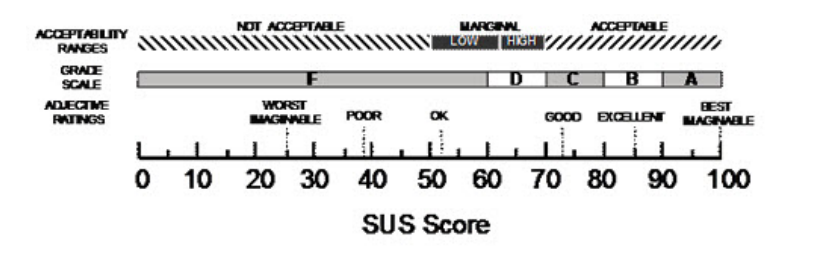
\includegraphics{pics/susscore}
		\caption{Nilai hasil evaluasi SUS \citep{paper.bangor}}
		\centering
	\end{figure}